% !TeX spellcheck = pl_PL
\documentclass[]{report}
\usepackage{etoolbox}
\usepackage{polski}
\usepackage[utf8]{inputenc}
\usepackage{geometry}
\usepackage{color,soul}
\usepackage{sidecap}
\usepackage{blindtext}
\usepackage{amsmath}
\usepackage{wrapfig}
\usepackage{csvsimple}
\usepackage[shortlabels]{enumitem}
\usepackage{tabularx}
\usepackage{makecell}
\usepackage{graphicx}
\usepackage{booktabs}
\usepackage{svg}
\graphicspath{{pics/}{../pics/}}

\begin{document}
\newgeometry{tmargin=2cm, bmargin=2cm, lmargin=1.6cm, rmargin=1.6cm}
\title{Raport\\
	\large Projekt Android}
\author{Eryk Dobrosz \\
	Marcin Gackowski \\
	Grzegorz Kacprowicz}

{\let\newpage\relax\maketitle}


\chapter*{Idea}
\quad Celem naszego projektu bylo dostarczenie aplikacji-gry, w której można łączyć się za pomocą sieci i rywalizować z przyjaciółmi. \textbf{Mad Mad Race} to gra, która składa się z serii krótkich wyścigów, gdzie zwycięża ten zawodnik, któremu uda się zdobyć najwięcej punktów ze wszystkich graczy. Gracz otrzymuje punkt wtedy i tylko wtedy, gdy ukończy wyścig jako pierwszy. \\
Głównym pomysłem jest, aby rozgrywki były krótkie i trwały około dwudziestu sekund oraz żeby było ich dużo, co ma nadać grze dynamiki, w odróżnieniu od modelu z jedną, długą rundą.

\chapter*{Użyte technologie}
\quad Gra napisana została na silniku \textbf{Unity} w wersji 2018.3.8 w języku \textbf{C\#}. Wykorzystaliśmy następujące biblioteki:
\begin{itemize}
	\item UNet - implementacja sieciowości, sprawnego łączenia się dwóch lub więcej urządzeń za pomocą sieci,
	\item Zenject - pomoc w ustrukturyzowaniu kodu, m. in. umożliwienie sprawnego zaimplementowania wzorca \textit{Dependency Injection}, polegającego na ograniczeniu zależności między poszczególnymi komponentami w projekcie.
\end{itemize}

Łączenie się graczy oparte jest na zasadzie host-klient w obrębie jednej sieci. Gracz hostujący musi podać IP, aby reszta graczy mogła do niego dołączyć. Możliwa jest też rozgrywka za pomocą \textbf{Wi-Fi Direct}. Zaimplementowane jest proste GUI, mające na celu usprawnić proces łączenia się, a w polu adresu IP wyświetlają się dostępne adresy.

\chapter*{Przebieg rozgrywki}
\quad Gdy za pomocą menu uda nam się połączyć z hostem (lub nim jesteśmy) zaczyna się właściwa rozgrywka. Możemy wyróżnić cztery stany gry:
\begin{enumerate}
	\item \textbf{Lobby} - jest to miejsce, w którym przebywają gracze, zanim zacznie się wyścig, a także gdzie trafiają po jego zakończeniu. To właśnie w tej fazie gracze mogą do siebie dołączać. Po dołączeniu zostaje im przydzielony unikalny identyfikator (nick) oraz i pojawia się on też w tablicy wynikowej w prawym dolnym rogu wraz z liczbą punktów (na początku zero). Aby przejść do następnej fazy gry, wszyscy obecni w lobby gracze muszą wyrazić gotowość - kliknąć na ekran. Pojawi się wtedy nad nimi "zielony ptaszek".
	\item \textbf{Odliczanie} - faza poprzedzająca każdy wyścig, która trwa dokładnie trzy sekundy i na ekranie wyświetlają się cyfry. Ruszyć z miejsca można wtedy, gdy licznik dojdzie do zera.
	\item \textbf{Wyścig} - główna faza gry, która jest opisana dokładniej poniżej.
	\item \textbf{Zakończenie} - każdemu graczowi wyświetlany jest napis z informacją o tym czy wygrał, czy też przegrał daną rundę. Gracz, który zwyciężył, otrzymuje punkt. Suma punktów każdego gracza jest widoczna w tabeli w prawym dolnym rogu. Ten stan gry trwa kilka sekund, po czym wszyscy gracze zostają przeniesieni z powrotem do lobby.
\end{enumerate}
W każdej z tych faz można kliknąć przycisk \textit{Exit} w lewym górnym rogu, który przenosi gracza z powrotem do menu, tym samym wyłączając go z gry. \\\\
Gdy wszyscy gracze w lobby wyrażą gotowość do gry, przenoszeni zostają na planszę z grą, gdzie każdy gracz pojawia się na początku losowo wybranego toru. Ilość torów jest zawsze o 2 większa od liczby graczy (teoretycznie może dołączyć ich dowolnie dużo).
Wyścig rozpoczyna się wraz z momentem zakończenia odliczania. Zaimplementowano także mechanizm \textit{boost}, który pozwala wystartować graczowi z pewną początkową prędkością, jeżeli kliknie on w odpowiednim momencie na ekran podczas odliczania (im bliżej końca odliczania został kliknięty ekran, tym większe przyspieszenie dostaje gracz - musi to być pierwsze kliknięcie w ekran, aby boost został naliczony).\\
Postać porusza się tylko do przodu i nie może się cofać. Prędkość gracza rośnie, gdy dotykamy ekranu. Prędkości nie można samemu zmniejszyć - jest to mechanizm, który ma na celu zachęcić gracza do rozważnego przyspieszania swojej postaci. Nie można też przyspieszać w nieskończoność - istnieje prędkość maksymalna. Aby skręcić, należy zrobić swipe w lewo lub w prawo. Gracze nie mogą wchodzić na siebie, tylko blokują się wzajemnie - jest to forma pewnego utrudnienia, zwiększająca jeszcze bardziej element rywalizacji. Plansza jest ograniczona i na jej końcu znajduje się meta. Dodatkowo na planszy generują się losowo przeszkody:
\begin{itemize}
	\item Kamień - zabija gracza. Kończy on wtedy swój bieg i musi czekać, aż runda się zakończy.
	\item Beczka - zmniejsza prędkość gracza do zera, ale nie zabija go.
\end{itemize}
Gra kończy się, gdy:
\begin{itemize}
	\item któryś gracz dobiegnie do mety - jest mu przyznawany punkt. Gracz, który jako drugi dobiegnie oraz kolejni już nie dostają punktu - liczy się tylko najszybszy z nich,
	\item nikt nie dobiegnie do mety, czyli wszyscy gracze zginą po drodze.
\end{itemize}
\begin{center}
	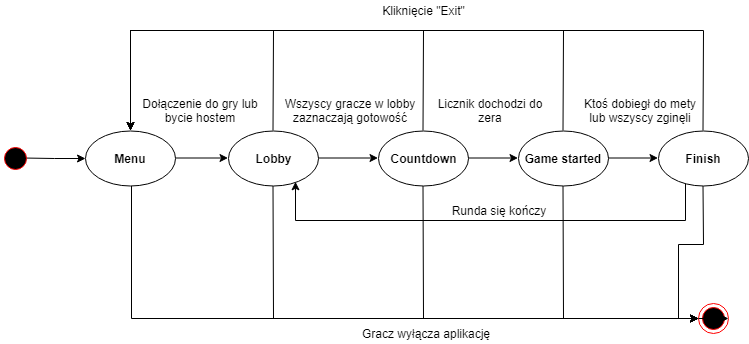
\includegraphics[width=0.9\textwidth]{game_cycle.png}
\end{center}

\end{document}
